\section[Marco Teórico]{CAPÍTULO 3:$\ \ \ \ $MARCO TEÓRICO} 

\subsection[Representación temporal y frecuencial de señales]{REPRESENTACIÓN TEMPORAL Y FRECUENCIAL DE SEÑALES}

El sonido se genera cuando un disturbio que se propaga por un
material elástico causa una alteración de la presión o un desplazamiento
de las partículas del material que puedan ser reconocidos por una persona o por un instrumento \cite{Beranek}. 
En este trabajo se manipulan señales de audio digitales, por lo cual se realiza un muestreo periódico de la señal de audio analógica. La distancia temporal entre dos muestras contiguas se determina según la frecuencia máxima que se desea representar, acorde al teorema de Nyquist \cite{openheim}. Entonces, una señal continua $x_{c}(t)$ que es muestreada a una frecuencia de $f_{s}$ muestras por segundo, produce una señal discreta $x[n]$ como se expresa en la ecuación \ref{eqn:discreta}.

\begin{equation}
\label{eqn:discreta}
	x[n] = x_{c}(nT_{s}) \qquad \qquad -\infty < n < \infty
\end{equation} 

En donde $T_{s}$ es el período de muestreo, y es equivalente al inverso de la frecuencia de muestreo $f_{s}$.
Partiendo de esta representación temporal discreta de la señal, se puede obtener una representación frecuencial (espectro) de la misma a partir de la Transformada Discreta de Fourier (DFT) \cite{openheim}. 
Dada una señal discreta $x[n]$ con $N$ muestras, su transformada discreta de Fourier se define como:

\begin{equation}
\label{eqn:DFT}
	X[k] = \sum_{n=0}^{N-1} x[n]e^{-jn2 \pi k/N} \qquad \qquad  k = 0, 1, 2,..., N-1
\end{equation} 

En donde $X$ es la transformada de Fourier discreta de $x$, y cada muestra de $X[k]$ es el resultado del producto interno entre $x$ y una exponencial compleja de frecuencia $2 \pi k/N$. La DFT es invertible, por lo cual es posible recuperar la señal $x[n]$ a partir de $X[k]$ utilizando la transformada discreta de Fourier inversa (IDFT):

\begin{equation}
\label{eqn:furier2}
	x[n] = {1}/{N}\sum_{k=0}^{N-1} X[k]e^{jnk2\pi/N} \qquad  0\leq n \leq N-1
\end{equation} 

Existen algoritmos eficientes para el cálculo de la DFT denominados algoritmos de transformada rápida de Fourier (FFT) \cite{fft}. Estos consiguen realizar el cálculo de la DFT reduciendo considerablemente la complejidad computacional (de $\textup{O}(N^{2})$ a $\textup{O}(Nlog(N))$).

\subsubsection{Transformada de corto término de Fourier (STFT)}

Las señales sonoras a analizar pueden ser no estacionarias. En este caso, la forma de onda de la señal nos brinda información del orden de aparición de los eventos sonoros, pero no sobre sus características frecuenciales. Por otro lado, la DFT nos permite tener información sobre la estructura frecuencial de la señal, pero resignando información sobre la evolución temporal. Entonces, para representar adecuadamente este tipo de señales tanto en tiempo como en frecuencia se utiliza la transformada de corto término de Fourier (STFT). La misma consiste en calcular la DFT sobre una ventana temporal que limita la cantidad de muestras a utilizar. Esta ventana se desplaza a lo largo de la señal, de manera tal que el resultado final pueda representar las características frecuenciales y sus variaciones en el tiempo. Matemáticamente, la STFT se define como: 

\begin{equation}
\label{eqn:STFT}
	X[t,k] = \sum_{n = 0}^{N-1}w[n]x[tH+n]e^{-j\frac{2 \pi k n}{N}}
\end{equation}

en donde:

\begin{itemize}
    \item $X[t,k]$ es la transformada de corto término de Fourier de $x[n]$.
    \item $t$ y $k$ son los indices temporales y frecuenciales respectivamente.
    \item $w[n]$ es la ventana utilizada.
    \item $N$ es el número de muestras de la ventana
    \item $H$ es el número de muestras que se desplaza la ventana. Se lo denomina tamaño de salto o \textit{hop size}, y determina el factor de solapamiento entre ventanas. 
\end{itemize}

En la Figura \ref{fig:stft_analisis} se ilustra el proceso descrito para la obtención de la STFT.

\begin{figure}[H]
  \centering{}
  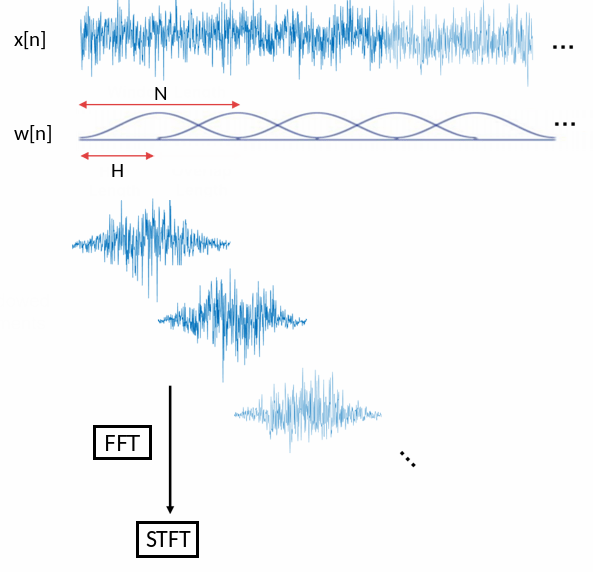
\includegraphics[scale=0.5]{stft_analisis.png}
  \caption{Proceso de obtención de la STFT. Extraído y adaptado de \cite{matlab}.}
  \label{fig:stft_analisis}
\end{figure}

El resultado de la STFT depende tanto de la señal bajo análisis como del tipo de ventana utilizada. Esto se debe a que la señal y la ventana se multiplican en el dominio del tiempo, lo que equivale a una convolución en frecuencia. Es decir que el espectro frecuencial de la señal se verá distorsionado por el espectro frecuencial de la ventana utilizada. Sabiendo esto, las ventanas se diseñan para controlar la distorsión espectral que producen sobre la señal bajo análisis. Existen dos tipos principales de distorsión espectral: el manchado espectral y la fuga espectral. El manchado espectral refiere a una pérdida de resolución en frecuencia y esta relacionado al ancho del lóbulo principal del espectro de la ventana utilizada. Por otro lado, la fuga espectral consiste en la aparición de componentes frecuenciales que no corresponden a la señal bajo análisis y esta relacionada a la amplitud relativa del lóbulo principal con respecto a los lóbulos secundarios. En la Figura \ref{fig:ventanas} se muestran algunas ventanas con sus respectivas respuestas en frecuencia.

\begin{figure}[H]
  \centering{}
  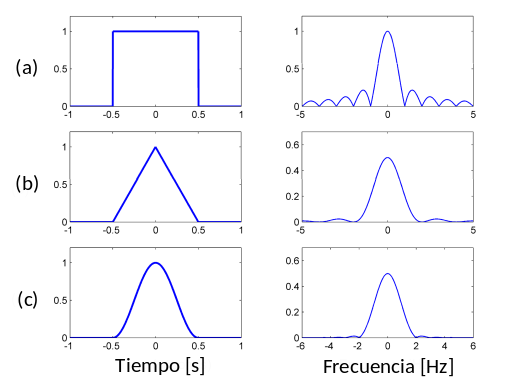
\includegraphics[scale=0.5]{ventanas.png}
  \caption{Ventanas \textbf{(a)} rectangular, \textbf{(b)} triangular y \textbf{(c)} Hann, con sus respectivas respuestas en frecuencia. Extraído de \cite{valerio}.}
  \label{fig:ventanas}
\end{figure}

% STFT como matriz compleja
EL resultado de aplicar la STFT es una matriz de números complejos. Dicha matriz puede descomponerse en componentes de magnitud y fase. Comúnmente, en tareas de procesamiento de audio, la información de fase se descarta y se trabaja únicamente con la magnitud. Tomando la magnitud de la STFT, las amplitudes suelen representarse en una escala de colores para producir una visualización como la que se muestra en la Figura \ref{fig:STFT} a la que se denomina espectrograma.

 \begin{figure}[H]
  \centering{}
  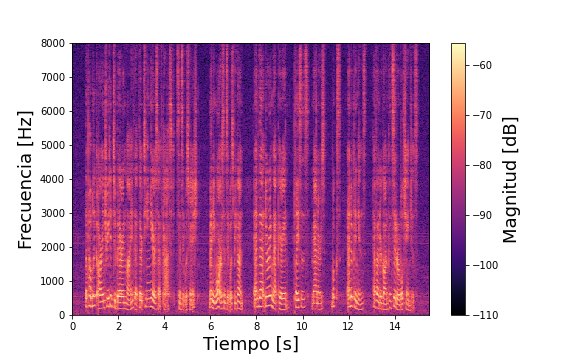
\includegraphics[scale=0.5]{STFT.png}
  \caption{Espectrograma de una señal de audio.}
  \label{fig:STFT}
\end{figure}

% porcentaje de solapamiento y su importancia  
La STFT es una transformación reversible. Para obtener una señal temporal partiendo de una STFT se aplica la técnica de solapamiento y suma (overlap-add). La misma consiste en calcular la IDFT para cada cuadro temporal de la STFT y sumar las señales resultantes aplicando el mismo desplazamiento que se utilizó en el proceso de análisis. En términos matemáticos, esta operación se define como:

\begin{equation}
\label{eqn:ISTFT}
	x[n] = \sum_{t=0}^{L-1}Shift_{tH}[\frac{1}{N}\sum_{k=0}^{N-1}X[t,k]e^{j\frac{2\pi kn}{N}}]
\end{equation}

En donde $L$ es la cantidad de cuadros temporales presentes en la STFT. Para que la reconstrucción de la señal sea correcta, la ventana utilizada tiene que cumplir con el criterio de solapamiento y suma constante (COLA):

\begin{equation}
\label{eqn:COLA}
		\sum_{t=0}^{L-1}w[n-tH] = \alpha \ \ \forall n \in  \mathbb{Z}
\end{equation}

donde $\alpha$ es una constante. Cuando $\alpha = 1$ la reconstrucción es perfecta. Para otros valores de $\alpha$ se deben aplicar compensaciones de amplitud sobre la señal reconstruida. La ventana de Hann cumple el criterio COLA siempre que la relación $\frac{N}{H}$ sea un número entero mayor a 1. En la Figura \ref{fig:solapa} se muestran ejemplos de diferentes grados de solapamientos. Se puede ver que cuando no se cumple la relación anteriormente mencionada entre el largo de la ventana y el tamaño de salto, se produce una modulación en la amplitud de la señal recuperada. 

 \begin{figure}[H]
  \centering{}
  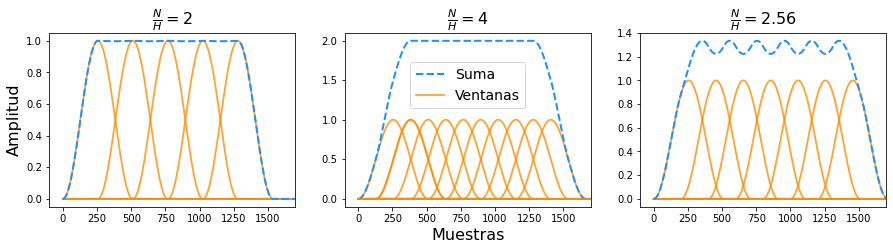
\includegraphics[scale=0.5]{solapamiento.png}
  \caption{Efecto del solapamiento entre ventanas en la STFT.}
  \label{fig:solapa}
\end{figure}

\subsection[Respuesta al impulso y reverberación]{RESPUESTA AL IMPULSO Y REVERBERACIÓN}

Si en un recinto se tiene una fuente sonora y un micrófono captando a una cierta distancia, las ondas sonoras emitidas se reflejan en las paredes del recinto y alcanzan el micrófono inmediatamente después que la onda sonora directa. Cada instancia de reflexión supone una disminución de la energía de la onda, principalmente causada por el efecto de absorción acústica de las superficies que producen las reflexiones. En un determinado tiempo, la energía sonora decaerá en todo el recinto hasta ubicarse por debajo del ruido de fondo. A este proceso se lo denomina reverberación. Al camino mas corto entre la fuente y el punto de captura se denomina camino directo, y a la relación de nivel entre la presión sonora que genera la onda propia del camino directo y la presión que genera el efecto de reverberación se lo conoce como relación directo-reverberado. 

Si el micrófono se ubica cerca de la fuente va a captar en mayor medida la señal correspondiente al camino directo, y una pequeña porción del sonido reverberado. Es decir, una relación directo-reverberado alta. A medida que el punto de captura se aleja de la fuente va a captar una menor cantidad del sonido correspondientemente al camino directo, mientras que el campo reverberado se mantendrá aproximadamente invariante. Esto se traduce en una disminución de la relación directo-reverberado. 
De esta manera, habrá una distancia específica para la cual el nivel de presión sonora generado por la fuente sera igual al nivel de presión sonora generado por el efecto de la reverberación. Esta distancia se conoce como distancia crítica. Esta depende tanto de las condiciones del recinto como de las características del micrófono. 

Si pensamos a la fuente y el micrófono dentro del recinto como un sistema, es de interés estudiar su respuesta al impulso $h(n)$ para poder calcular una serie de parámetros que describan las características acústicas del recinto. Como su nombre lo indica, la respuesta al impulso equivale a la respuesta del sistema cuando se lo excita con un impulso infinitamente angosto (delta de Dirac). La respuesta al impulso será diferente para cada par de puntos fuente-receptor dentro del recinto.   


La Figura \ref{fig:rir} muestra una respuesta al impulso junto con un esquema temporal de la misma. En dicho esquema podemos identificar 3 partes: primero, el nivel de sonido directo (producido por la onda que viaja a través del camino directo), las reflexiones tempranas (cuyo limite temporal vendrá definido por las características propias de cada recinto) y por último la cola reverberante. Se puede distinguir la parte de reflexiones tempranas y la cola reverberante partiendo de la suposición de que las reflexiones tempranas ocurren en un proceso determinístico, siendo altamente sensibles a pequeños cambios en la geometría del recinto, mientras que la cola reverberante es mas bien un proceso estocástico, y al depender de un mayor número de reflexiones no varía drásticamente frente a pequeños cambios de geometría. 

\begin{figure}[H]
  \centering{}
  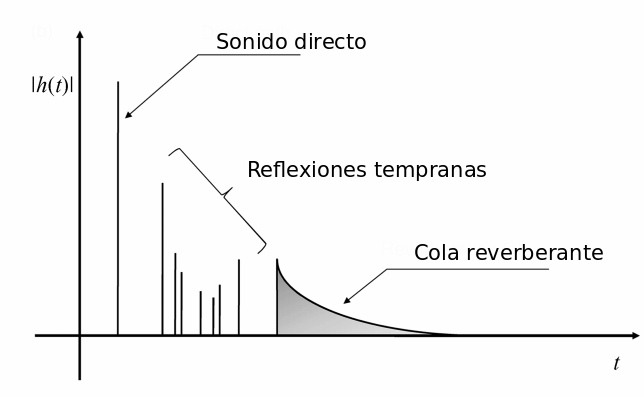
\includegraphics[scale=0.30]{rir.png}
  \caption{Secciones temporales de una respuesta al impulso. Extraído de \cite{rir}.}
  \label{fig:rir}
\end{figure}

Idealmente, el micrófono captura una señal que corresponde a la convolución entre la respuesta al impulso del recinto y la señal fuente, como se ve en la ecuación \ref{eqn:impulso}. Esto equivale a una multiplicación en el dominio de la frecuencia de acuerdo con la transformada de Fourier, como se ve en la ecuación \ref{eqn:frecuencia}.  


\begin{equation}
\label{eqn:impulso}
	x(t) = h(t) * s(t)
\end{equation} 

\begin{equation}
\label{eqn:frecuencia}
	X(f) = H(f)S(f)
\end{equation} 

De esta manera se puede ver que la respuesta al impulso conserva toda la información sobre la influencia de la reverberación del recinto sobre la señal captada por el micrófono. 

La respuesta al impulso de un recinto real se mide actualmente utilizando una técnica de barrido frecuencial \cite{sinesweep}. Además, existen modelos geométricos que se utilizan para determinar la respuesta al impulso de manera analítica. Los principales son el modelo de trazado de rayos \cite{raytracing} y el modelo fuente imagen \cite{sourceimage}. Estos modelos asumen la propagación del sonido como rayos en lugar de ondas. En la Figura \ref{fig:analitic_rir} se ilustran ambos modelos. 

\begin{figure}[H]
  \centering{}
  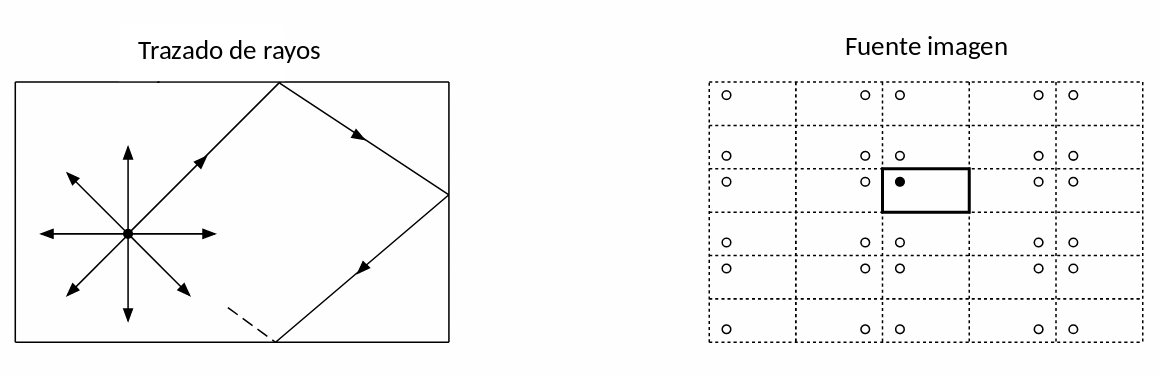
\includegraphics[scale=0.40]{rir_analitic.png}
  \caption{Modelos analíticos de cálculo de la respuesta al impulso de un recinto. Extraído de \cite{rir}.}
  \label{fig:analitic_rir}
\end{figure} 

El trazado de rayos consiste en considerar un punto de fuente que emite radialmente. La longitud de los caminos de cada rayo y los coeficientes de absorción acústica de las superficies del recinto se utilizan para determinar la respuesta al impulso del recinto. Por otro lado, el modelo de fuente imagen se basa en el principio de que una reflexión especular puede ser definida geométricamente espejando la fuente respecto del plano de reflexión. De esta forma se genera una imagen especular de la fuente por cada superficie de reflexión, y esto se aplica de manera recursiva. La suma de todas las fuentes imágenes con sus respectivos retardos y atenuaciones conforman la respuesta al impulso estimada del recinto.



\subsubsection{Relación directo-reverberado (DRR)}

Es un descriptor acústico que se aplica sobre respuestas al impulso. Se define según la ecuación \ref{eqn:DRR} en la cual $h(n)$ representa la respuesta al impulso discreta obtenida. Los índices desde cero hasta $n_{d}$ representan las muestras correspondientes a la señal directa, y las muestras que continúan luego de $n_{d}$ representan solo la reverberación producida por las reflexiones. 

\begin{equation}
\label{eqn:DRR}
	DRR  [dB]= 10 Log_{10}(\frac{\sum_{n=0}^{n_d}h^{2}(n)}{\sum_{n=n_{d}+1}^{\infty}h^{2}(n)}) 
\end{equation}

Este parámetro es dependiente de la distancia entre el punto emisor y receptor, y del tiempo de reverberación del recinto. Como esta definición inicialmente se piensa en un dominio continuo, la primera intuición es pensar que el camino directo está fielmente representado por la mayor magnitud en la parte temprana de la respuesta al impulso. Sin embargo, esto solo es correcto cuando el tiempo de propagación entre la fuente y el receptor es un múltiplo entero del período de muestreo. Por esto, trabajar con frecuencias de muestreo finitas (dominio discreto) en general deriva en que la representación del camino directo se produzca a través de una función seno cardinal ($Sinc$) correspondiente a la ventana de muestreo, centrada de acuerdo al retardo correspondiente al tiempo de propagación. En cambio, cuando se trata de respuestas al impulso sintéticas, el camino directo puede ser computado de forma separada del resto. Es decir, se puede determinar con exactitud el aporte del campo directo y del campo reverberado, lo que permite el cálculo del parámetro $DRR$ con una mayor exactitud. 




\subsection[Inteligibilidad y parámetros de calidad de percepción]{INTELIGIBILIDAD Y PARÁMETROS DE CALIDAD DE PERCEPCIÓN}

Para caracterizar la señal del habla propagándose en condiciones reverberantes se utilizan métricas objetivas derivadas de la respuesta al impulso del recinto en cuestión, como por ejemplo el tiempo de reverberación o la relación energética entre la señal directa y el campo reverberado. En cambio, al considerar el proceso de dereverberación de estas señales las respuestas al impulso requieren ser estimadas, lo que usualmente conduce a una caracterización de baja calidad. Además, los algoritmos de dereverberación pueden introducir artefactos audibles a la señal voz, los cuales no son contemplados por las respuestas al impulso estimadas. Es por esto que es preciso utilizar métodos de medida de calidad basados en la señal dereverberada. Las pruebas subjetivas son el método más confiable para evaluar la calidad percibida de una señal de habla dereverberada. Sin embargo, este método es costoso y requiere mucho tiempo, por lo cual se vuelve inviable su aplicación para procesamientos en tiempo real. Para aplicaciones prácticas se definieron entonces métodos objetivos de medición de calidad basados en la señal dereverberada como reemplazo de las pruebas subjetivas. Estos métodos consisten en algoritmos que de manera objetiva y repetible buscan estimar la calidad percibida de la señal, por lo cual, un método resulta efectivo cuando logra obtener una alta correlación con las respuestas subjetivas. Estos métodos se clasifican en intrusivos o no intrusivos, dependiendo de si requieren o no una señal de referencia para realizar la estimación. Poder contar con una señal de referencia para realizar estas estimaciones es usualmente una dificultad, por lo cual se presta mayor interés en aquellos métodos no intrusivos. 

\subsubsection{Relación energía de modulación de voz a reverberación}

Este parámetro de medida de calidad para señales dereverberadas se basa en obtener características de la reverberación partiendo del espectro de modulación de la señal \cite{SRMR}. La formulación de este parámetro se basa en el hecho de que la cola reverberante de una respuesta al impulso puede ser modelada como ruido blanco Gaussinano exponencialmente amortiguado. Esta característica puede ser explotada en el análisis del espectro de modulación de la señal bajo análisis para obtener descriptores del efecto de la reverberación.

\subsubsection{Inteligibilidad objetiva de corto termino extendida}
Este parámetro está basado en características extraídas a partir de la correlación de corto término entre la señal limpia y la señal procesada. Es aplicable para evaluar aquellos procesos que realizan transformaciones no lineales \cite{ESTOI}. Su funcionamiento se basa en aplicar una ventana de análisis de $384$ $ms$ en las envolventes de amplitud de las subbandas de la señal analizada. Estas ventanas temporales se aplican en pos de contemplar frecuencias de modulación que son relevantes para la inteligibilidad. En estos lapsos temporales se calculan coeficientes de correlación espectrales que son luego promediados. De esta manera, este parámetro puede ser interpretado en términos de una descomposición ortogonal de espectrogramas energéticamente normalizados que son luego ordenados de acuerdo a su contribución a la inteligibilidad estimada. 

\subsubsection{Relación señal a distorsión}

Este descriptor fue ampliamente utilizado en tareas de separación de fuentes y refuerzo de señales de habla. Esta basado en el cómputo de la relación señal a interferencia (SIR), y en la relación señal a artefacto (SAR) \cite{SAR}. En las tareas de dereverberación, estas medidas pueden ser interpretadas como proporcionales a la supresión de componentes reverberantes tardías e inversamente proporcionales a la distorsión en la señal del habla, respectivamente. Contemplando estos valores, el parámetro final mide la calidad general de la señal dereverberada.  

\subsection[Redes neuronales y algoritmos de aprendizaje profundo]{REDES NEURONALES Y ALGORITMOS DE APRENDIZAJE PROFUNDO}
Las redes neuronales artificiales son herramientas de modelado computacional que comparten algunas propiedades con el funcionamiento de las neuronas biológicas  \cite{neurona}. Estas conforman el estado del arte actual para la resolución y modelado de problemas de alta complejidad en diversas disciplinas \cite{ANN_intro}. 

\subsubsection{La neurona artificial}
El bloque básico de los modelos de aprendizaje profundo es la neurona artificial. El esquema de una neurona artificial se puede ver en la Figura \ref{fig:neurona}. Sus componentes principales son: 

\begin{figure}[H]
  \centering{}
  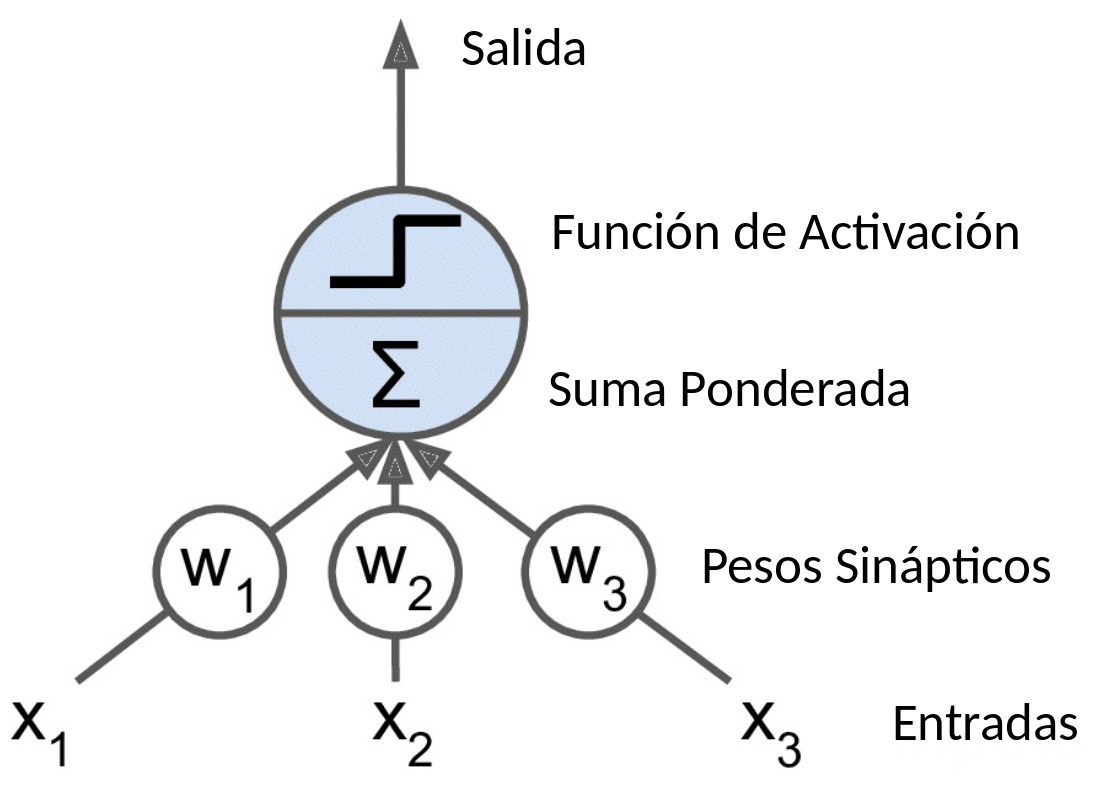
\includegraphics[scale=0.30]{neurona.png}
  \caption{Esquema de neurona artificial. Extraído de \cite{dragon}.}
  \label{fig:neurona}
\end{figure}

\begin{itemize}
    \item \textbf{Entradas}: son los datos que van a ser procesados en esta unidad.
    \item \textbf{Pesos sinápticos}:son parámetros asociados a cada entrada que se van ajustando durante la etapa de entrenamiento. 
    
    \item \textbf{Suma ponderada}: Sintetiza la entrada a la función de activación. Consiste en el producto interno entre el vector de entradas y el vector de pesos sinápticos. Matemáticamente, se expresa como:
    
    \begin{equation}
\label{eqn:suma_ponderada}
	\sum_{i=1}^{n}x_{i}w_{i}
\end{equation}
    
    donde $x$ son las entradas, $w$ los pesos sinápticos y $n$ el número de entradas.
    \item \textbf{Función de activación}: Función que se aplica a la salida de la suma ponderada, y genera la salida de la neurona. La misma introduce alinealidades en la neurona, haciendo que el modelo resultante sea no lineal. Algunos ejemplos de funciones de activación se pueden ver en la Figura \ref{fig:activación}. 
    
    \item \textbf{Salida}: Es el resultado de aplicar el proceso completo al conjunto de entradas. En una red neuronal, esta salida puede ser la entrada de una o varias unidades subsiguientes. 
\end{itemize}


\begin{figure}[H]
  \centering{}
  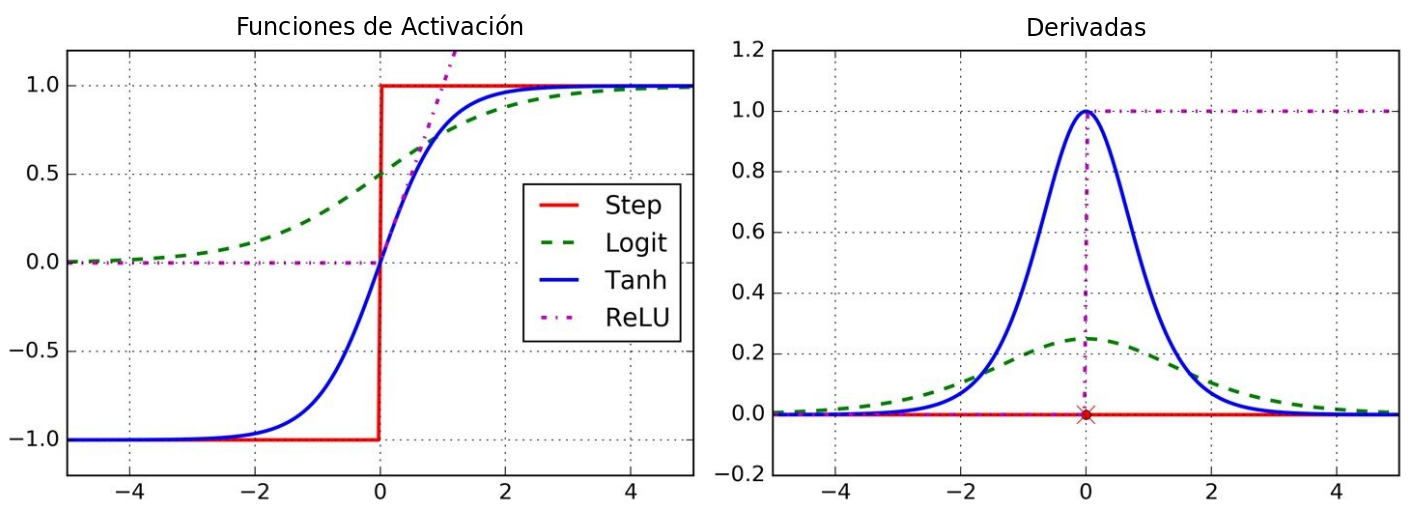
\includegraphics[scale=0.30]{activacion.png}
  \caption{Funciones de activación y sus derivadas. Extraído de \cite{lagartija}.}
  \label{fig:activación}
\end{figure}

\subsubsection{Modelos basados en redes neuronales}

Una red neuronal suele organizarse en capas, las cuales poseen una cierta cantidad de neuronas. El comportamiento de la red neuronal se define en base a su arquitectura. La arquitectura depende principalmente de:
\begin{itemize}
\item Número de capas.
\item Número de neuronas por capas.
\item Tipos de conexiones entre las capas.
\end{itemize}

La red neuronal con alimentación hacia adelante fue el primer tipo de red neuronal implementado. En esta red neuronal, la información fluye en un solo sentido, desde la entrada hacia la salida. 

Una de las redes neuronales mas estudiadas es la red neuronal multicapas con alimentación hacia adelante (feed-forward multilayer neural network). Esta consta de una capa de entrada, una o varias capas ocultas, y una capa de salida. Cada capa puede contener un número distinto de neuronas, y cada capa se encuentra completamente conectada a la capa adyacente. Esta red neuronal es capaz de representar cualquier función dado un número suficiente de neuronas. Un ejemplo de esta red se ilustra en la Figura \ref{fig:red}.

\begin{figure}[H]
  \centering{}
  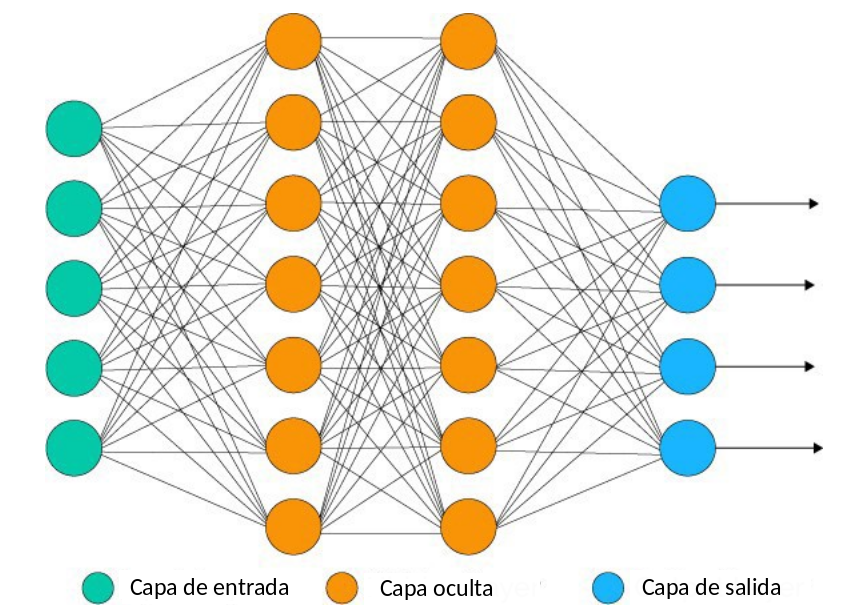
\includegraphics[scale=0.35]{red.png}
  \caption{Ejemplo de red neuronal multicapa con alimentación hacia adelante.}
  \label{fig:red}
\end{figure}

Frecuentemente se cataloga a las redes neuronales multicapas como algoritmos de aprendizaje profundo. Esto se debe a que contienen múltiples capas de procesamiento no lineal que aprenden diferentes niveles de representación formando una jerarquía de características, desde un nivel de abstracción mas bajo a uno mas alto \cite{franchute}.  

\subsubsection{Entrenamiento y aprendizaje}

Los algoritmos de aprendizaje por máquina se entrenan a partir del procesamiento de datos. Cuando se trata de un modelo de aprendizaje supervisado, los datos de entrenamiento se presentan de a pares $(x,y)$ en donde $y$ es el valor objetivo o la salida que se espera obtener para el valor de entrada $x$. En el contexto del entrenamiento de una red neuronal, se define al aprendizaje como la búsqueda de una determinada configuración de los parámetros entrenables de la red que produzcan que la entrada $x$ genere la salida $y$. En general, inicialmente las entradas van a generar salidas $\hat{y}$ aleatorias que difieren del valor objetivo $y$. Entonces, es necesario tener una medida de esta diferencia. De eso se encarga la función de costo (también denominada función objetivo o función de pérdida).

La función de costo recibe las salidas de la red y las salidas esperadas, y luego calcula una medida de error a partir de una función matemática. Esta función se escoge de acuerdo a la tarea que se busca realizar. Entonces, para cada estimación de la red, la función de costo otorga un puntaje que explica cuan lejos está el valor estimado del valor objetivo.  

El paso siguiente en el proceso de entrenamiento es utilizar la salida de la función de costo como una señal de realimentación para poder ajustar los parámetros entrenables de la red neuronal (pesos sinápticos, umbrales, etc) de manera tal de minimizar la función de costo. Esta tarea es realizada por la función de optimización. La misma aplica el algoritmo de propagación del error hacia atrás para computar el gradiente de la función de costo respecto a los parámetros entrenables de la red neuronal. En base a este gradiente y al valor de tasa de aprendizaje definido en la función de optimización, se puede determinar como modificar los parámetros entrenables para lograr disminuir el error de salida. Este bucle de entrenamiento se ilustra en el esquema de la Figura \ref{fig:esquema}. Repetir este ciclo un número suficiente de veces conduce a la convergencia del valor de error. 

\begin{figure}[H]
  \centering{}
  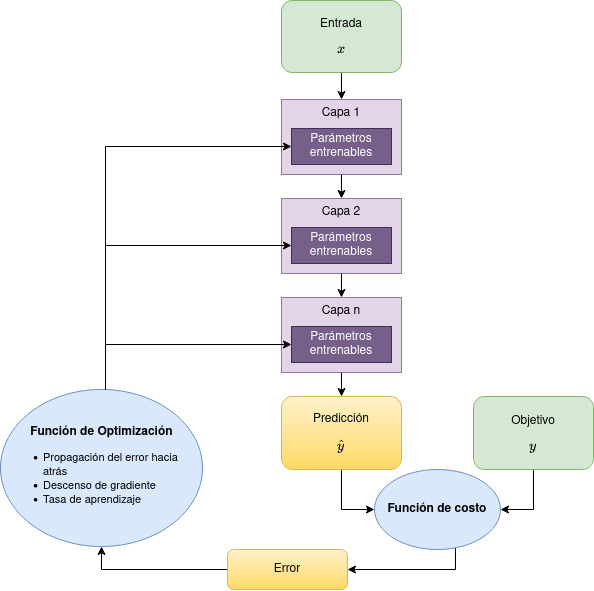
\includegraphics[scale=0.65]{esquema_red.jpg}
  \caption{Diagrama de flujo del bucle de entrenamiento de una sistema de red neuronal.}
  \label{fig:esquema}
\end{figure}


En este trabajo el conjunto de datos de entrenamiento se segmenta en lotes. En cada iteración de entrenamiento la red neuronal recibe un lote, lo procesa, aplica la función de costo y ajusta los parámetros de cada capa. Cuando la red procesó todos los lotes que componen el conjunto de datos de entrenamiento se dice que transcurrió una época. El proceso de entrenamiento depende en cierta medida del tamaño de los lotes \cite{franchute}. Si consideramos la curva de la función de costo de un parámetro como la de la Figura \ref{fig:costo_curva}, vemos que existen mínimos locales y mínimos globales a lo largo de la misma. En el proceso de entrenamiento se busca minimizar este valor de costo. Si se toman lotes muy pequeños, lo que se traduce en desplazamientos pequeños a lo largo de esta curva, se corre el riesgo de quedar confinado en un mínimo local. De igual manera, un conjunto demasiado grande produciría saltos demasiado grandes en comparación a las fluctuaciones de esta curva, haciendo que se obtengan valores de costo aleatorios. 

\begin{figure}[H]
  \centering{}
  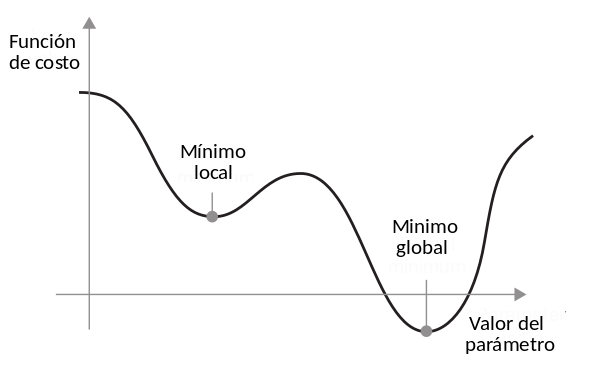
\includegraphics[scale=0.35]{costo_curva.png}
  \caption{Curva de costo para un parámetro}
  \label{fig:costo_curva}
\end{figure}

El orden en el que los datos son presentados ante el modelo puede influenciar positiva o negativamente en el resultado final del entrenamiento. Existen técnicas de optimización que se desarrollaron partiendo de cualidades propias del aprendizaje en seres humanos y animales, como el hecho de que el aprendizaje resulta mejor cuando las instancias de aprendizaje están organizadas en un orden significativo, añadiendo gradualmente mayor cantidad de conceptos y por ende una mayor complejidad. Esta idea se traslada al entrenamiento de algoritmos de aprendizaje profundo con el desarrollo de una estrategia denominada aprendizaje por currículum \cite{cv}. La misma consiste en seleccionar cuales datos y en que orden presentarlos al sistema durante el aprendizaje, de manera de guiar el entrenamiento para que inicialmente se aprendan los conceptos mas sencillos del problema, e ir gradualmente aumentando el grado de complejidad de la tarea. El aprendizaje por currículum se define como una estrategia de optimización global. Dependiendo de la tarea sobre la que se aplica, puede lograr en menor o mayor medida que un sistema logre un mejor nivel de generalización así como también llegar al punto de convergencia en un menor tiempo de entrenamiento.


Por último, la segmentación de los datos que la red neuronal recibe y procesa en cada etapa del desarrollo también influye en el desempeño de la misma. El objetivo final del sistema es alcanzar un grado de generalización que le permita procesar adecuadamente instancias de datos que no hayan sido reveladas ante la red en la etapa de entrenamiento. Por esto, el conjunto total de los datos se divide en tres subgrupos: 

\begin{itemize}
\item\textbf{Conjunto de entrenamiento}: Este conjunto de datos es el que se utiliza en la etapa de entrenamiento para optimizar los parámetros de la red. Aquí se concentra el mayor volumen de datos.

\item\textbf{Conjunto de validación}: Sobre este conjunto se mide el desempeño del sistema a lo largo de su entrenamiento. Los resultados obtenidos del procesamiento de este conjunto sirven para ajustar variables que requieren ser especificadas de manera previa al entrenamiento. Estas variables se denominan hiper parámetros.
 
\item\textbf{Conjunto de prueba}: Este conjunto es el que se utiliza para medir el rendimiento final del sistema. Como contiene instancias que no fueron utilizadas en las etapas de entrenamiento y ajuste de parámetros, el análisis del procesamiento de este conjunto sirve para medir el nivel de generalización que el sistema logró alcanzar. 

\end{itemize}

Durante el entrenamiento pueden ocurrir dos fenómenos indeseados: el sobreajuste y el subajuste. 
El sobreajuste refiere al caso en que el modelo obtenga muy buenos resultados sobre los datos de entrenamiento, pero malos resultados sobre los datos de valdiación y evaluación. Es decir, el modelo no alcanzó el grado de generalización pretendido, y memorizó las instancias de entrenamiento. Esto ocurre cuando la complejidad del modelo es muy alta en comparación a la complejidad de la tarea que busca resolver.
El subajuste, en cambio, hace referencia a un error elevado en la etapa de entrenamiento. Esto ocurre cuando el modelo es muy simple, o carece de la complejidad necesaria para realizar la tarea. 

Existen varias estratégias para lidiar con los problemas de sobreajuste, como por ejemplo:

\begin{itemize}
\item\textbf{Aumento de datos de entrenamiento}: Proporcionar más datos a la etapa de entrenamiento produce una mejora en la capacidad de generalización del modelo. De todos modos, obtener mas datos no siempre es posible, y por eso existen técnicas de aumentación, que consisten en manipular datos ya existentes para generar datos nuevos.  

\item\textbf{Dropout}: Es una técnica de regularización que consiste en anular aleatoriamente un determinado número de activaciones de una capa durante el entrenamiento \cite{drop}. Es equivalente a entrenar un numero menor de neuronas, lo que se traduce en una reducción de la complejidad del modelo.  

\item\textbf{Interrupción temprana del entrenamiento}: Esta estrategia consiste en detener el entrenamiento antes de que el modelo comience a sobreajustar los datos \cite{bengio}.  Para determinar el punto en el que el modelo empieza a sobreajustar, comúnmente se monitorea el error que produce el modelo sobre el conjunto de validación a medida que transcurre el entrenamiento.
\end{itemize}

Otra técnica importante que se utiliza en este trabajo es la normalización por lotes \cite{batchnorm}. Esta consiste en normalizar las entradas de una capa, restando la media y dividiendo por el desvío estándar del lote de datos actual. Esto produce que el entrenamiento sea mas veloz (se logra la convergencia del error mas rápidamente) y estable. 

\subsubsection{Redes neuronales convolucionales}

Las redes neuronales convolucionales emergen del estudio de la corteza visual del cerebro animal \cite{animales}. En los últimos años, estas estructuras fueron utilizadas para resolver tareas visuales complejas (análisis de imágenes). 
El bloque básico de las redes neuronales convolucionales es la capa convolucional. La misma posee las siguientes características:

\begin{itemize}

\item \textbf{Campo receptivo limitado}: las neuronas que conforman la capa convolucional no están conectadas a todas las entradas, sino que solo se conectan con una porción de las mismas que se denomina campo receptivo. Esto hace que se modelen estructuras locales, es decir, presentes dentro de este campo receptivo.  

\item \textbf{Parámetros compartidos}: los pesos sinápticos de las neuronas se comparten. Por esto, los patrones aprendidos por las neuronas son invariantes a la traslación. Esto quiere decir que si se aprende de un patrón ubicado en un lugar específico del volumen de entrada, este mismo patrón puede luego ser identificado en cualquier otra ubicación de la entrada.

\item \textbf{Convolución}: se aplican filtros de convolución sobre las entradas, que comúnmente son imágenes. Si bien la literatura utiliza el término convolución, matemáticamente se realiza una correlación cruzada. La Figura \ref{fig:convolucion} muestra en que consiste este proceso, y como el filtro se desplaza sobre las entradas para generar las salidas. En cada paso, el filtro se multiplica por una sección de la imagen de entrada (producto interno) y el resultado corresponde a un solo valor en la imagen de salida. Las salidas de una capa convolucional se denominan mapas de características.  

\end{itemize}


El funcionamiento a partir de campos receptivos y el hecho de que los parámetros se comparten entre neuronas producen que las capas convolucionales sean mas eficientes en términos de cantidad parámetros a entrenar. 


\begin{figure}[H]
  \centering{}
  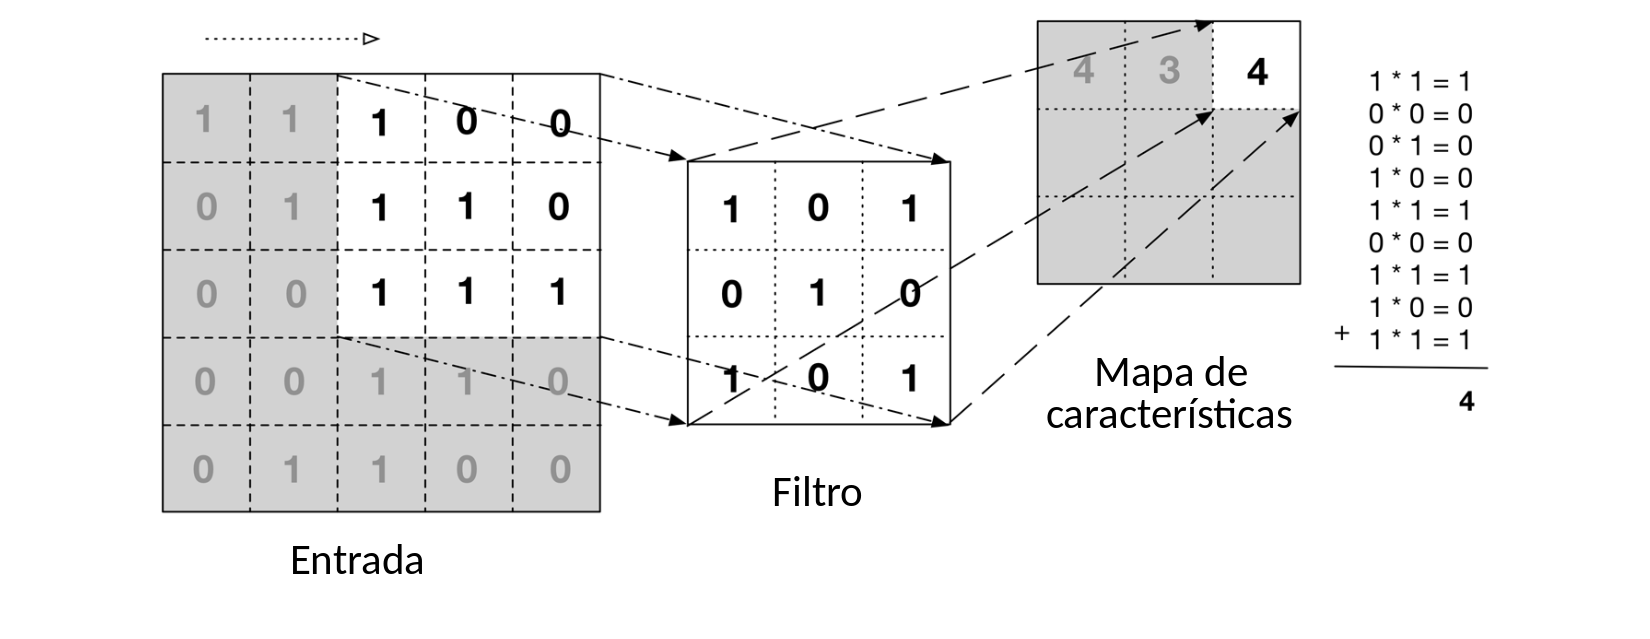
\includegraphics[scale=0.25]{convolucion.png}
  \caption{Funcionamiento de un filtro de convolución. Extraído de \cite{dragon}.}
  \label{fig:convolucion}
\end{figure}

De esta manera, una capa convolucional aplica uno o varios filtros bidimensionales sobre la imagen de entrada, generando mapas de características que representan la presencia del patrón del filtro a lo largo de la imagen, como se puede apreciar en la Figura \ref{fig:numerito}. En este tipo de capas, el aprendizaje se traduce en determinar la forma de los filtros que se deben aplicar para conseguir los resultados esperados. 

\begin{figure}[H]
  \centering{}
  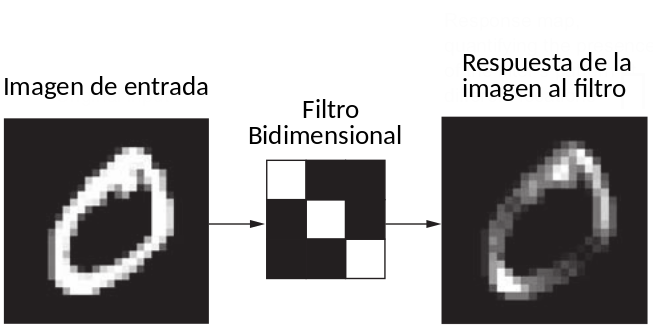
\includegraphics[scale=0.35]{filtro.png}
  \caption{Representación de la aplicación de un filtro bidimensional sobre una imagen.}
  \label{fig:numerito}
\end{figure}

Los hiperparámetros que se deben definir en cada capa convolucional son: 

\begin{itemize}
\item\textbf{Tamaño del filtro}: Define el tamaño del campo receptivo de cada unidad de procesamiento de la capa. Valores comunes son $3x3$ o $5x5$. En la Figura \ref{fig:variables_conv} se ve un ejemplo de un filtro de tamaño $3x3$.

\item\textbf{Tamaño del salto}: Determina la distancia horizontal y vertical entre campos receptivos de dos unidades contiguas. Hacer que este valor sea mayor a uno permite reducir las dimensiones de la imagen de entrada al atravesar la capa convolucional. Esto se puede apreciar en la Figura \ref{fig:variables_conv} en donde se aplica un tamaño de salto igual a dos (tanto en sentido vertical como horizontal). 

\item\textbf{Relleno de ceros}: Cuando se pretende mantener invariables las dimensiones de entrada y salida de una capa convolucional, se suele aplicar un relleno con ceros en los contornos de la imagen. La cantidad de ceros agregados dependerá de las características del filtro a aplicar. Aplicar un relleno de ceros produce un fenómeno denominado efecto de borde \cite{lagartija}. 

\item\textbf{Cantidad de filtros aplicados}: El número de filtros convolucionales que se aplican sobre la entrada. Es equivalente al número de mapas de características que se generan. 

\end{itemize}

\begin{figure}[H]
  \centering{}
  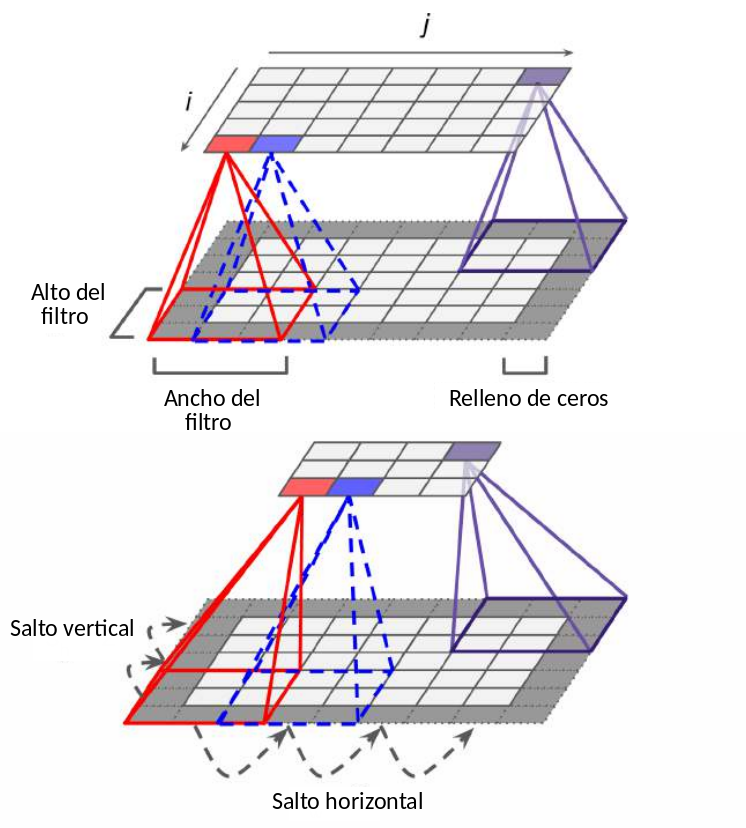
\includegraphics[scale=0.35]{filtrosconv.png}
  \caption{Parámetros de procesamiento en capas convolucionales. Extraído de \cite{lagartija}.}
  \label{fig:variables_conv}
\end{figure}


Para el análisis de imágenes, estas capas se concatenan de manera que la primera capa no contempla cada píxel de la imagen, sino que solo se enfoca un número acotado de píxeles que caen dentro de su campo receptivo. De igual manera, las capas subsiguientes se enfocan en las salidas de un conjunto acotado de neuronas de la capa precedente. Este funcionamiento se ilustra en la Figura \ref{fig:convnet}. 

\begin{figure}[H]
  \centering{}
  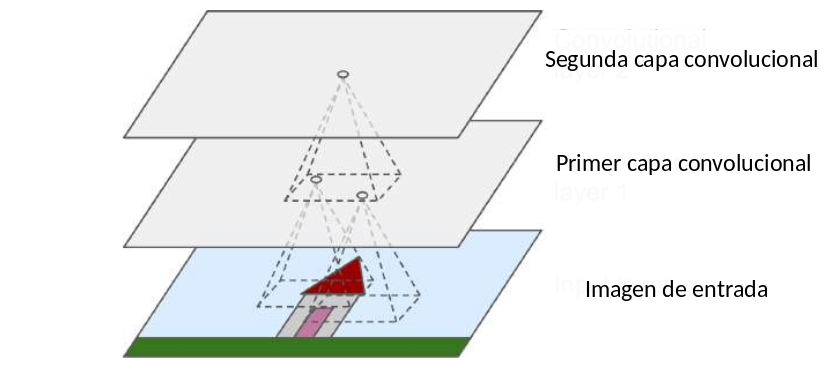
\includegraphics[scale=0.35]{convnet.png}
  \caption{Capas convolucionales con campos receptivos locales rectangulares}
  \label{fig:convnet}
\end{figure}

Formar esta estructura le permite a la red aprender diferentes patrones estructurales locales de manera jerárquica \cite{lagartija}. En conclusión, a diferencia de las redes completamente conectadas, las redes convolucionales logran la generalización de conceptos visuales complejos a partir de una menor cantidad de parámetros, distribuidos estratégicamente a lo largo de la arquitectura.  

\subsubsection{Autoencoders}

Un autoencoder es una arquitectura de red neuronal cuyo objetivo es copiar su entrada en su salida. El esquema básico de un autoencoder se puede observar en la Figura \ref{fig:autoencoder}, donde $x$ representa a las variables de entrada, $r$ representa las variables de salida y $h$ representa las variables latentes. 

\begin{figure}[H]
	\centering{}
	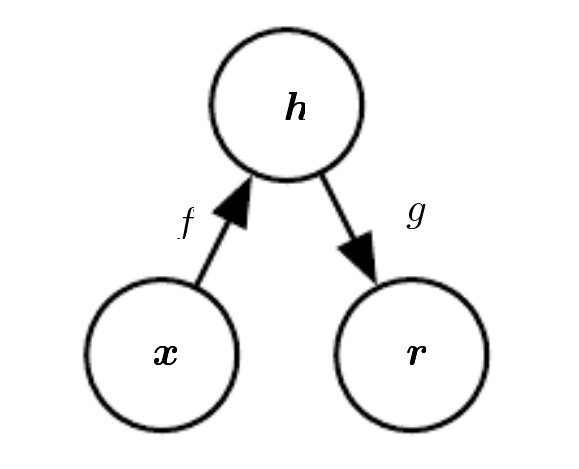
\includegraphics[scale=0.3]{autoencoder.png}
	\caption{Estructura general de un autoencoder.}
	\label{fig:autoencoder}
\end{figure}

El esquema  se compone de tres partes fundamentales: 
\begin{itemize}
\item Una función de codificación $f$ en donde las dimensiones de la variable de entrada se comprimen, idealmente descartando información irrelevante para la reconstrucción de la entrada. De esta forma, se logra reducir la dimensionalidad de la variable de entrada, conservando solo la información más relevante.

\item Un espacio latente $h$ (o espacio de representación), el cual es la representación comprimida de la entrada que genera la codificación f.

\item Una función de decodificación en donde se aplica el proceso inverso que en la codificación, expandiendo las dimensiones tomadas del espacio latente para reconstruir la señal de entrada. 
\end{itemize}

Comúnmente, este tipo de arquitecturas se entrenan restringiendo o condicionando los datos de entrada, para que la red se vea obligada a priorizar que aspectos de la entrada deben copiarse, lo que a menudo implica aprender propiedades útiles de los datos.



\subsection[Dereverberación por filtrado temporal-frecuencial]{DEREVERBERACIÓN POR FILTRADO TEMPORAL-FRECUENCIAL}

\subsubsection{Máscaras de amplitud}

Existen numerosas maneras de representar las señales de audio para dereverberarlas. En la actualidad, los espectrogramas son la más utilizada ya que su cálculo es rápido y sencillo, son interpretables, es posible invertirlos y pueden ser fácilmente aprovechados por modelos de aprendizaje profundo como las redes neuronales convolucionales. Partiendo de una señal con reverberación, se extrae una representación en tiempo-frecuencia a partir de transformaciones como la transformada de corto término de Fourier (STFT). Una vez obtenido este espectrograma, lo que se busca es descifrar el proceso necesario para obtener un nuevo espectrograma que se corresponda con la señal anecoica (descartando el efecto de la reverberación). Entonces, el proceso de dereverberación se puede resumir a la estimación de un filtro variable con el tiempo que se aplica sobre el espectrograma con reverberación. Estudios previos afirman que la fase no aporta información significativa para estas tareas de mejora del habla \cite{fase1}\cite{fase2}, por lo cual se suelen realizar estos procesos únicamente sobre la magnitud de los espectrogramas, utilizando la información de fase del audio original. Considerando esto, el proceso de dereverberación se reduce a la expresión de la ecuación \ref{eqn:dereverb}, en donde $STFT_{Y}$ es la magnitud del espectrograma de la señal anecoica, $STFT_{X}$ es la magnitud del espectrograma de la señal con reverberación y $M$ es la máscara ideal que representa el filtrado en el dominio tiempo-frecuencia. En otras palabras, la magnitud del espectro de la señal dereverberada se obtiene aplicando la máscara ideal sobre la magnitud del espectrograma de la señal con reverberación. 
 
\begin{equation}
\label{eqn:dereverb}
	STFT_{Y}(t,f)= M(t,f) STFT_{X}(t,f) 
\end{equation}

Considerando que el espectro reverberado tendrá siempre mayor amplitud que el espectro anecóico, se trasladan los rangos de ambos espectros al intervalo $(0, 1]$. De esta manera, las máscaras resultantes estarán dentro del mismo intervalo. Este proceso de escalado de las entradas, resulta beneficioso para los modelos de redes neuronales artificiales \cite{lagartija}. Luego, la red neuronal tiene el objetivo de estimar la máscara ideal a partir del espectrograma reverberado. En la Figura \ref{fig:red_estim} se muestra un diagrama de cómo se estructura el sistema y las señales disponibles para lograr estimar la máscara de manera indirecta. El espectrograma con reverberación ingresa a la red neuronal artificial, la cual procesa esta entrada y produce una salida intermedia de las mismas dimensiones que la entrada. Luego, esta salida intermedia se multiplica con el espectrograma de entrada y el resultado es comparado con el espectrograma sin reverberación, mediante la función de costo. De esta manera, los pesos de la red neuronal se van a modificar en pos de que la salida del sistema sea lo más semejante posible al espectro sin reverberación. Cuando la función de costo tienda a cero, esto significará que la salida de la red neuronal tiende a igualarse con una máscara ideal, que al aplicarse sobre el espectrograma reverberado produce el espectrograma anecóico. 

\begin{figure}[H]
  \centering{}
  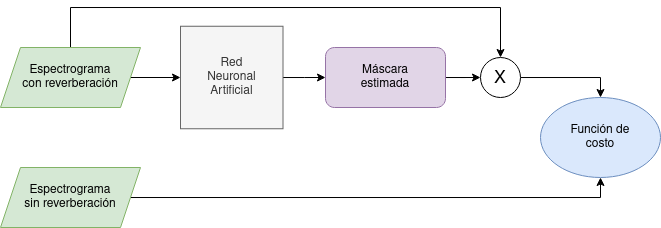
\includegraphics[scale=0.60]{estimacion_mascara.png}
  \caption{Disposición de las entradas y salidas del modelo para la estimación de las máscaras de amplitud}
  \label{fig:red_estim}
\end{figure}
  


\subsubsection{Síntesis de audio a partir de espectrogramas}

En este trabajo, como en muchas otras tareas de procesamiento de audio (y procesamiento de señales en general), se lleva a cabo la siguiente secuencia de pasos:

\begin{enumerate}
\item Tomar una señal en el dominio del tiempo $x[n]$ y convertirla en un espectrograma $X[t,f]$ a través de la STFT.
\item Modificar el espectrograma $X[t,f]$ para obtener $\hat{X}[t,f]$. 
\item Convertir el espectrograma modificado $\hat{X}[t,f]$ nuevamente a una señal en el dominio del tiempo $\hat{x}[n]$ a través de la ISTFT.
\end{enumerate}

El último paso de la lista conlleva un problema, ya que ciertos procesos pueden generar espectrogramas que no sean consistentes, es decir, que no haya ninguna señal en el dominio del tiempo cuyo espectrograma sea el generado. Para solucionar esta cuestión se desarrollaron algoritmos que buscan estimar una señal temporal cuyo espectrograma sea el más cercano posible al espectrograma que se quiere invertir. Este es el caso del algoritmo propuesto por Griffin y Lim \cite{griffinlim}. El algoritmo consiste en un bucle iterativo que busca minimizar el error cuadrático medio entre el espectrograma de la señal estimada y el espectrograma modificado. En la Figura \ref{fig:griffin} se muestra un diagrama de bloques que explica el funcionamiento básico del algoritmo. 

\begin{figure}[H]
  \centering{}
  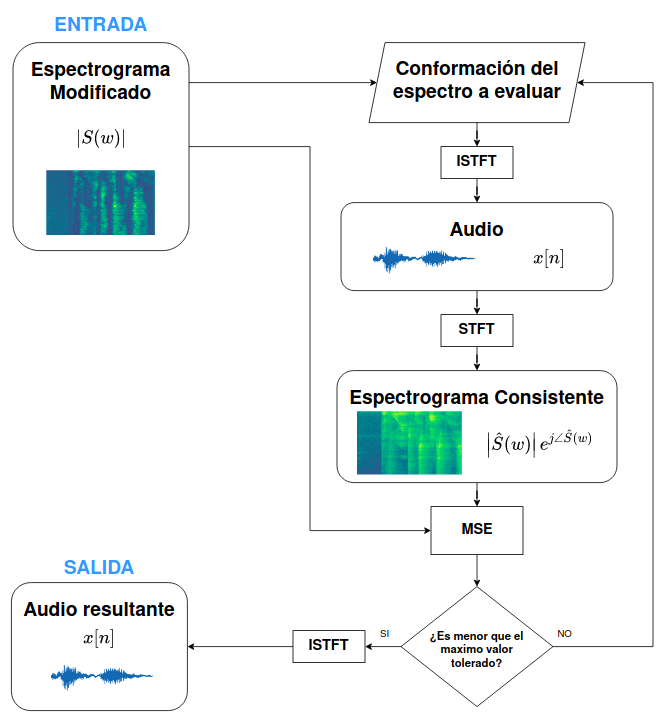
\includegraphics[scale=0.40]{griffin.png}
  \caption{Diagrama en bloques del algoritmo de Griffin-Lim.}
  \label{fig:griffin}
\end{figure}

La magnitud del espectrograma de entrada $\left | \hat{S}[t,f] \right |$ inicialmente se combina con una fase aleatoria para formar un espectrograma complejo. Si se cuenta con una estimación previa de la fase, esta puede utilizarse en lugar de la fase aleatoria al iniciar el proceso. Luego, el espectrograma complejo conformado se antitransforma obteniendo una señal de audio, la cual vuelve a ser transformada obteniéndose un nuevo espectrograma complejo $\left | S[t,f] \right |e^{j\angle S[t,f]}$. Este espectrograma es consistente, pues deriva de la transformación de una señal de audio real. Se puede probar que combinar esta fase resultante $\angle S[t,f]$ con el espectrograma modificado de entrada $\left | \hat{S}[t,f] \right |$ disminuye el error cuadrático entre los espectrogramas evaluados (es decir, entre el espectrograma consistente y el inconsistente). Entonces, se combina la fase consistente con la magnitud del espectrograma de entreda y se vuelve a repetir todo el proceso.   Se debe definir un criterio para determinar cuando dejar de iterar, y tomar al espectrograma consistente como el resultado final del proceso para antitransformarlo y obtener  $\hat{x}[n]$. Un criterio podría ser calcular la convergencia espectral al final de cada iteración, y definir un valor de tolerancia. De esta manera, el bucle se repite hasta que la diferencia entre los espectrogramas evaluados sea menor que un valor definido como tolerancia. Otro criterio, por ejemplo, podría ser directamente fijar un número de iteraciones a realizar a partir de el cual se asume la convergencia del espectro resultante. De igual manera se podrían definir otros criterios. 

